% Preamble
\documentclass[compress,aspectratio=169]{beamer}

%% Packages
\usepackage{amsmath}
\usepackage{graphicx}
\usepackage{xcolor}
\usepackage{tikz}
\usepackage{amssymb}
\usetikzlibrary{shapes, shadows, arrows,arrows.meta}
\usetikzlibrary{positioning}
\usepackage{hyperref}
\usepackage{mathtools}
\usepackage{pgfplots}
\usepackage{multicol}
%% Commands
\def\changemargin{\list{}{\rightmargin.2\linewidth\leftmargin.2\linewidth}\item[]}
\let\endchangemargin=\endlist

%% Theme
\usepackage[scaled]{helvet}
\renewcommand\familydefault{\sfdefault}
\usepackage[T1]{fontenc}

\setbeamertemplate{navigation symbols}{}
\setbeamertemplate{frametitle}{
	\vspace{.5in}
	\raggedright\insertframetitle%
}
\setbeamertemplate{bibliography item}{\insertbiblabel}
\setbeamercolor{frametitle}{fg=black}
\setbeamercolor{title}{fg=black}
\setbeamertemplate{itemize item}{\color{gray}$\blacktriangleright$}
\setbeamertemplate{enumerate item}{\color{gray}$\blacktriangleright$}
\setbeamercolor{normal text}{fg=darkgray}
\setbeamercolor{bibliography item}{fg=gray}
\setbeamercolor{bibliography entry author}{fg=black}
\setbeamercolor{bibliography entry title}{fg=darkgray}
\setbeamercolor{bibliography entry authors}{fg=darkgray}
\setbeamercolor{bibliography entry location}{fg=gray}
\setbeamercolor{bibliography entry note}{fg=gray}
\setbeamercolor{bibliography entry journal}{fg=gray}

\definecolor{myred}{RGB}{255, 42, 42}
\definecolor{mygreen}{RGB}{113, 200, 55}
\definecolor{myblue}{RGB}{42, 127, 255}

%% PGFPlot settings
\pgfplotsset{compat = newest}
\pgfplotsset{every axis/.append style={
			label style={font=\tiny},
			tick label style={font=\tiny}
		}}

% Metadata
\title{Signal processing for SSVEP BCI}
\author{NeuroTech Leuven}
\titlegraphic{
\includegraphics[width=.1\textwidth]{ntxl.png}\hskip.1in
\includegraphics[width=.1\textwidth]{kul.png}}

% Document
\begin{document}
\frame{
	\vskip0pt plus 1filll
		{\usebeamerfont{title}\usebeamercolor[fg]{title}\inserttitle}
	\bigskip

	\insertauthor \bigskip

	\insertdate \bigskip

	\inserttitlegraphic
	\vskip0pt plus 1filll

}

\frame{
	\frametitle{Neuroimaging modalities}

	\centering
	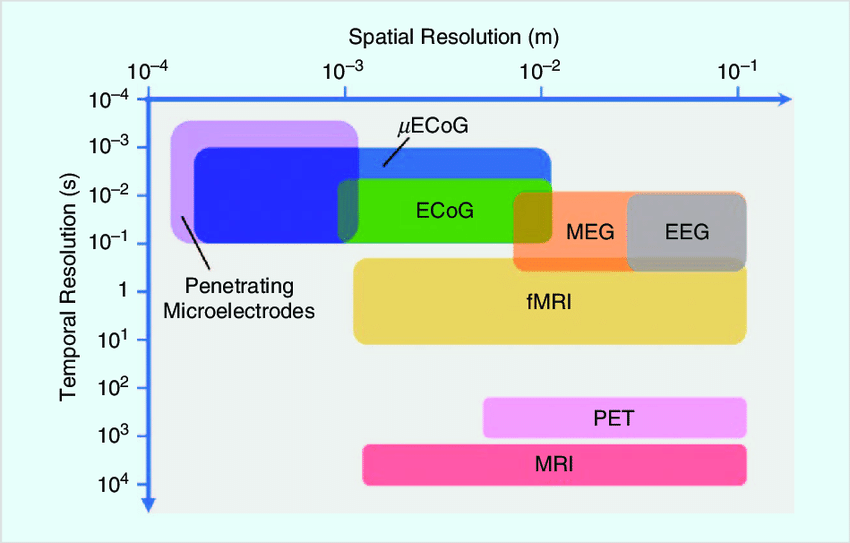
\includegraphics[width=.6\textwidth]{modalities.png}

	\bigskip

	\small Anish \textit{et al.} (2018)
}
\frame{
	\frametitle{BCI paradigms}

	\centering
	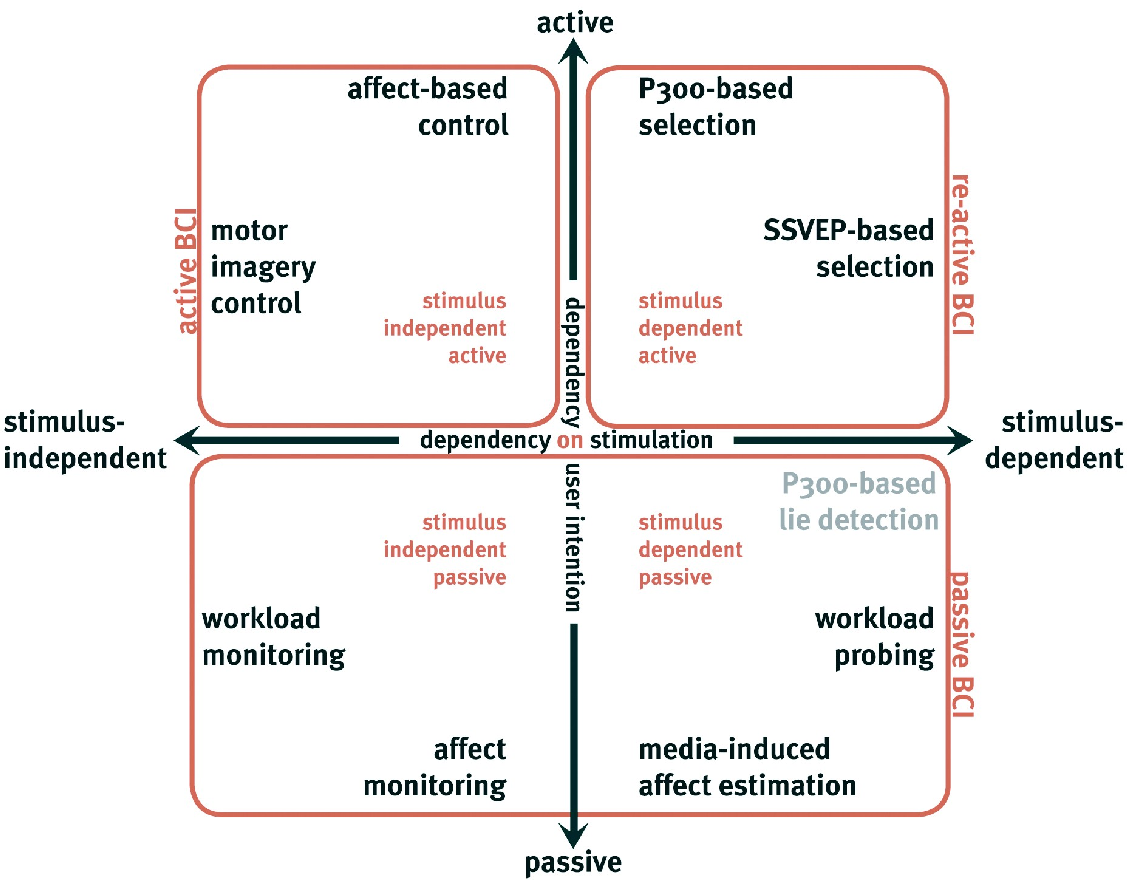
\includegraphics[width=.5\textwidth]{paradigms}

	\bigskip

	\small M\"uhl \textit{et al.} (2014)

}\frame{
	\frametitle{Steady State Visually Evoked Potentials}

	If a stimulus oscillates at a specific frequency, an oscillation at the
	same frequency will also appear in the brain activity of the occipital
	lobe.

	\centering
	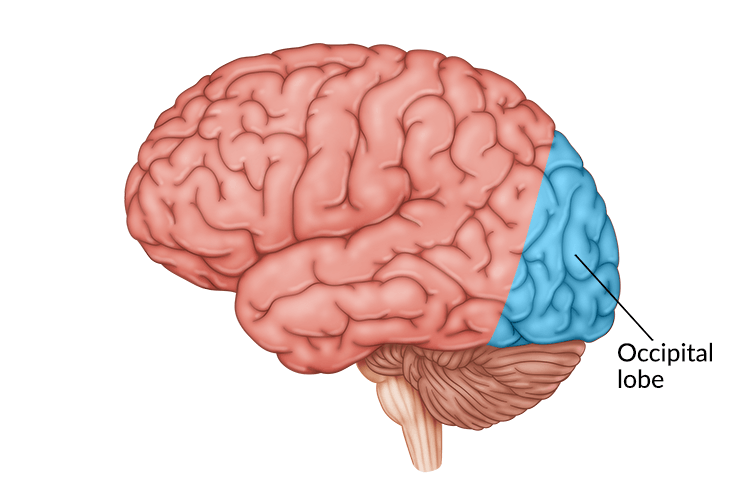
\includegraphics[width=.5\textwidth]{occipital_lobe.png}
}

\frame{
	\frametitle{SSVEP BCI}
	\centering
	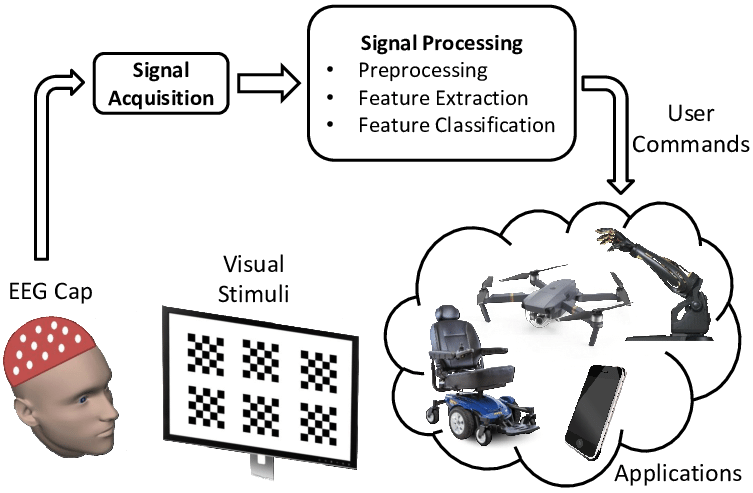
\includegraphics[width=.6\textwidth]{ssvep.png}
}


\frame{
	\frametitle{This workshop}
	\centering
	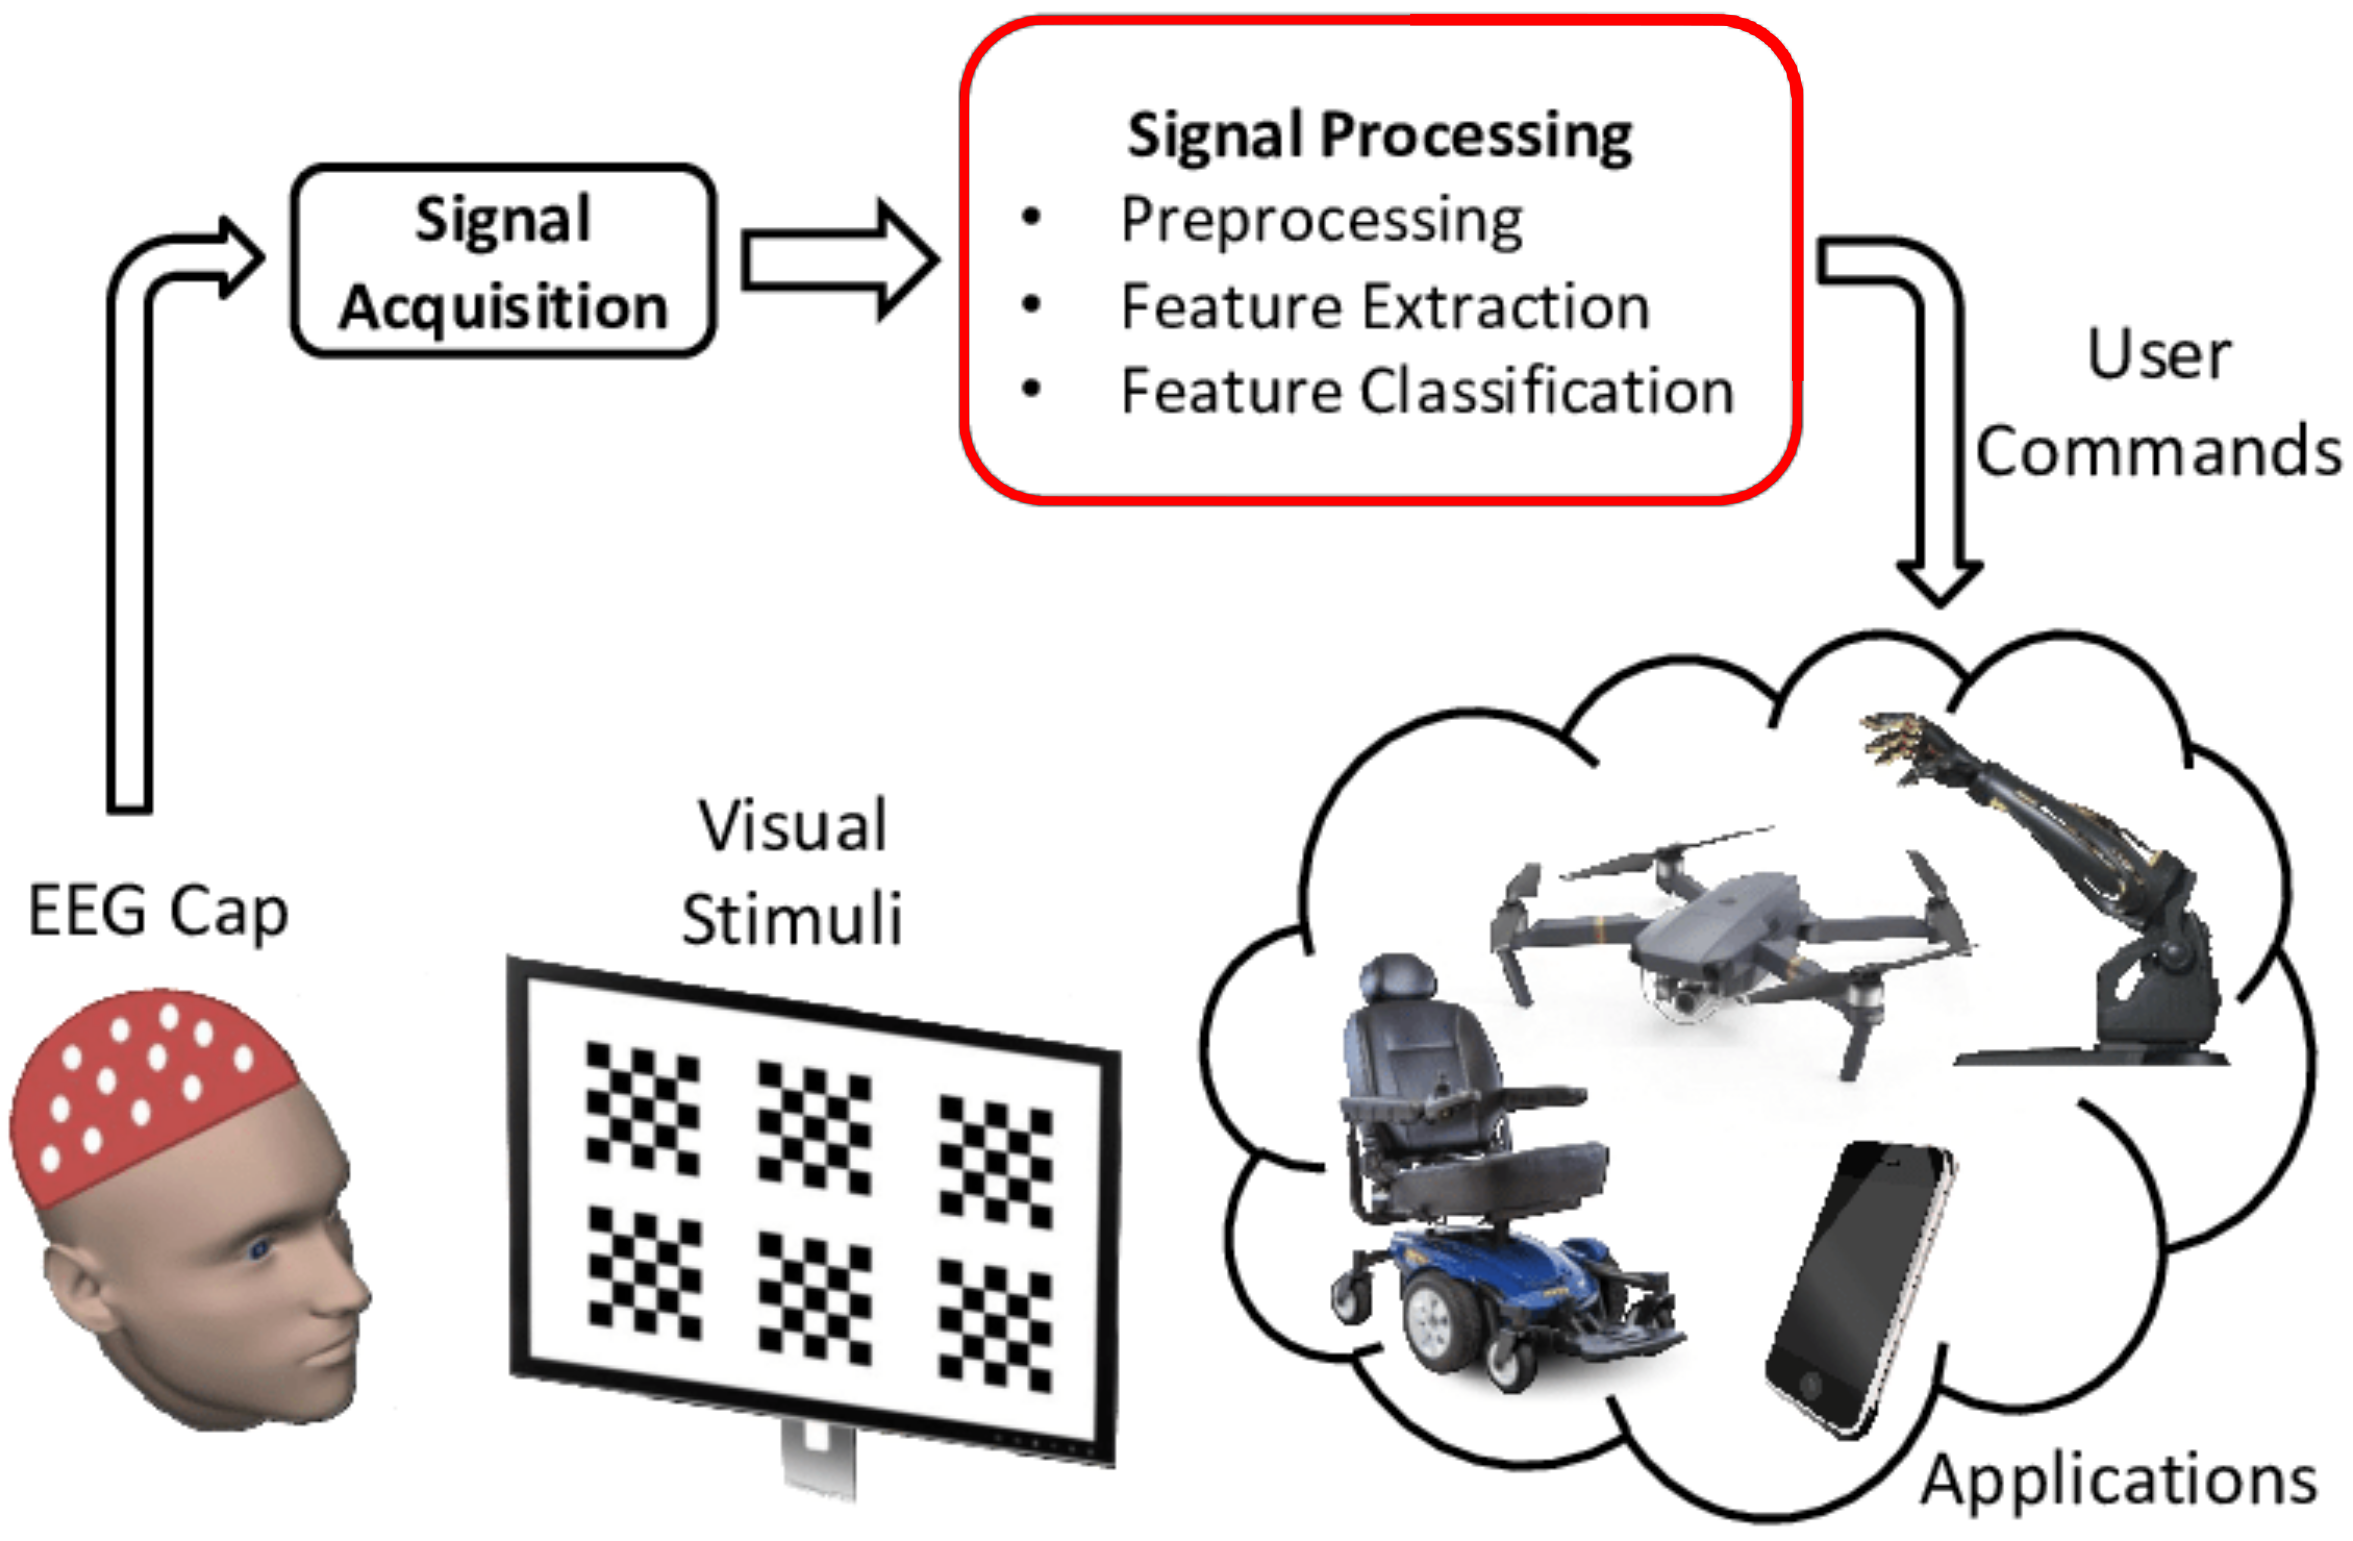
\includegraphics[width=.6\textwidth]{ssvep_workshop.png}
}
\frame{
	\frametitle{The Fourier transform}

	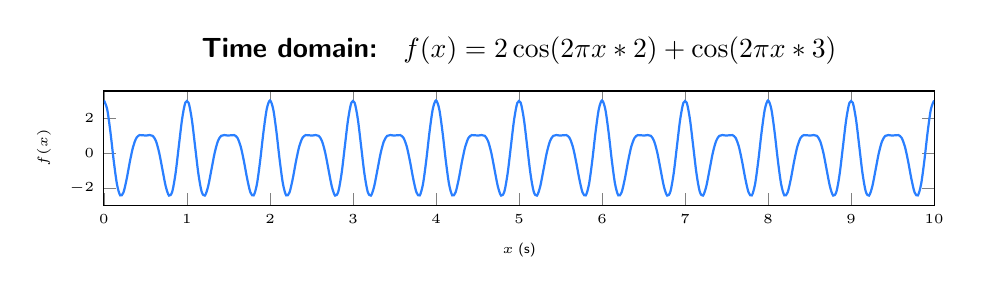
\begin{tikzpicture}
		\begin{axis}[
				width=\textwidth,
				height=.25\textwidth,
				xmin=0, xmax=10,
				xlabel={$x$ (s)},
				ylabel={$f(x)$},
				title={\textbf{Time domain: }
						$f(x)=2\cos(2\pi x*2) +
							\cos(2\pi x*3)$}
			]
			\addplot[
				domain=0:10,
				samples=256,
				smooth,
				thick,
				color=myblue,
			]{2*cos(deg(2*x*pi*2)) + cos(deg(2*x*pi*3))};
		\end{axis}
	\end{tikzpicture}
	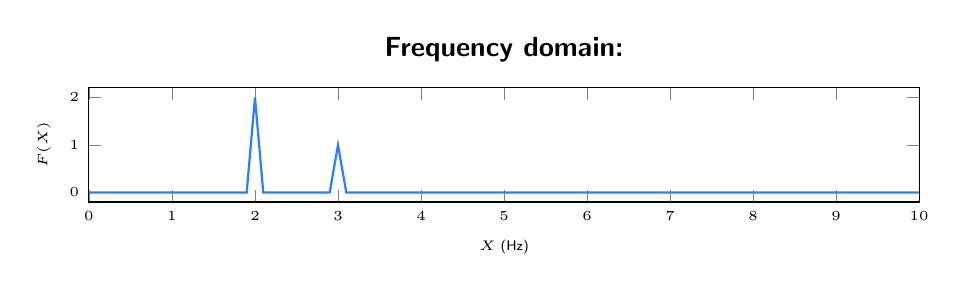
\begin{tikzpicture}
		\begin{axis}[
				width=\textwidth,
				height=.25\textwidth,
				xmin=0, xmax=10,
				xlabel={$X$ (Hz)},
				ylabel={$F(X)$},
				title={\textbf{Frequency domain: }}
			]
			\addplot[
				color=myblue,
				thick,
			]coordinates{(0,0)(1.9,0)(2,2)(2.1,0)(2.9,0)(3,1)(3.1,0)(10,0)};
		\end{axis}
	\end{tikzpicture}
}

\frame{
	\frametitle{Filtering}
	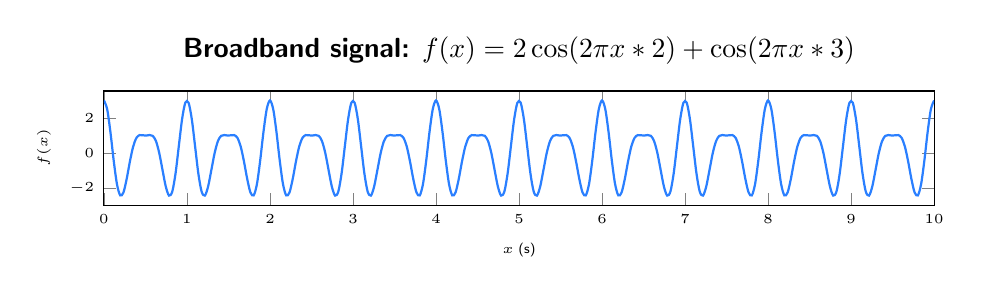
\begin{tikzpicture}
		\begin{axis}[
				width=\textwidth,
				height=.25\textwidth,
				xmin=0, xmax=10,
				xlabel={$x$ (s)},
				ylabel={$f(x)$},
				title={\textbf{Broadband signal:}
						$f(x)=2\cos(2\pi x*2) +
							\cos(2\pi x*3)$}
			]
			\addplot[
				domain=0:10,
				samples=256,
				smooth,
				thick,
				color=myblue,
			]{2*cos(deg(2*x*pi*2)) + cos(deg(2*x*pi*3))};
		\end{axis}
	\end{tikzpicture}
	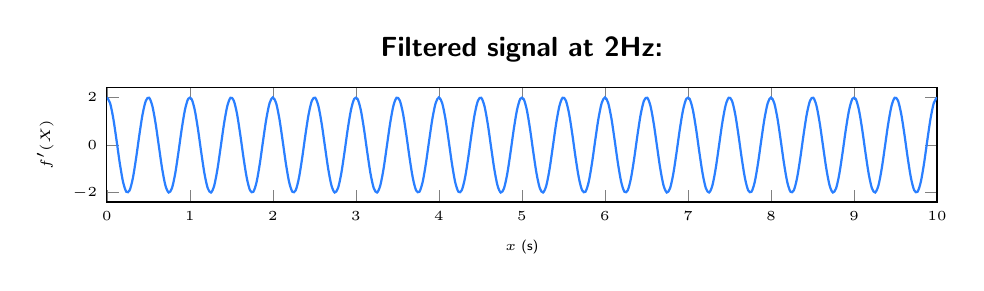
\begin{tikzpicture}
		\begin{axis}[
				width=\textwidth,
				height=.25\textwidth,
				xmin=0, xmax=10,
				xlabel={$x$ (s)},
				ylabel={$f'(X)$},
				title={\textbf{Filtered signal at 2Hz:}}
			]
			\addplot[
				domain=0:10,
				samples=256,
				smooth,
				thick,
				color=myblue,
			]{2*cos(deg(2*x*pi*2))};
		\end{axis}
	\end{tikzpicture}

}

\frame{
	\frametitle{Filtering}
	\begin{changemargin}
		\begin{columns}[t]
			\begin{column}{.5\linewidth}
				Apply a single filter:
				\begin{itemize}
					\item Single frequency filter
					\item Band-pass filter
					\item Band-stop filter
					\item Notch filter
				\end{itemize}
			\end{column}%
			\begin{column}{.5\linewidth}
				Apply a time-frequency transform:
				\begin{itemize}
					\item Filterbank
					\item Wavelet transform,
					\item Multitaper filtering
					\item \ldots
				\end{itemize}
			\end{column}
		\end{columns}
	\end{changemargin}
}


\frame{
	\frametitle{The EEG spectrum}
	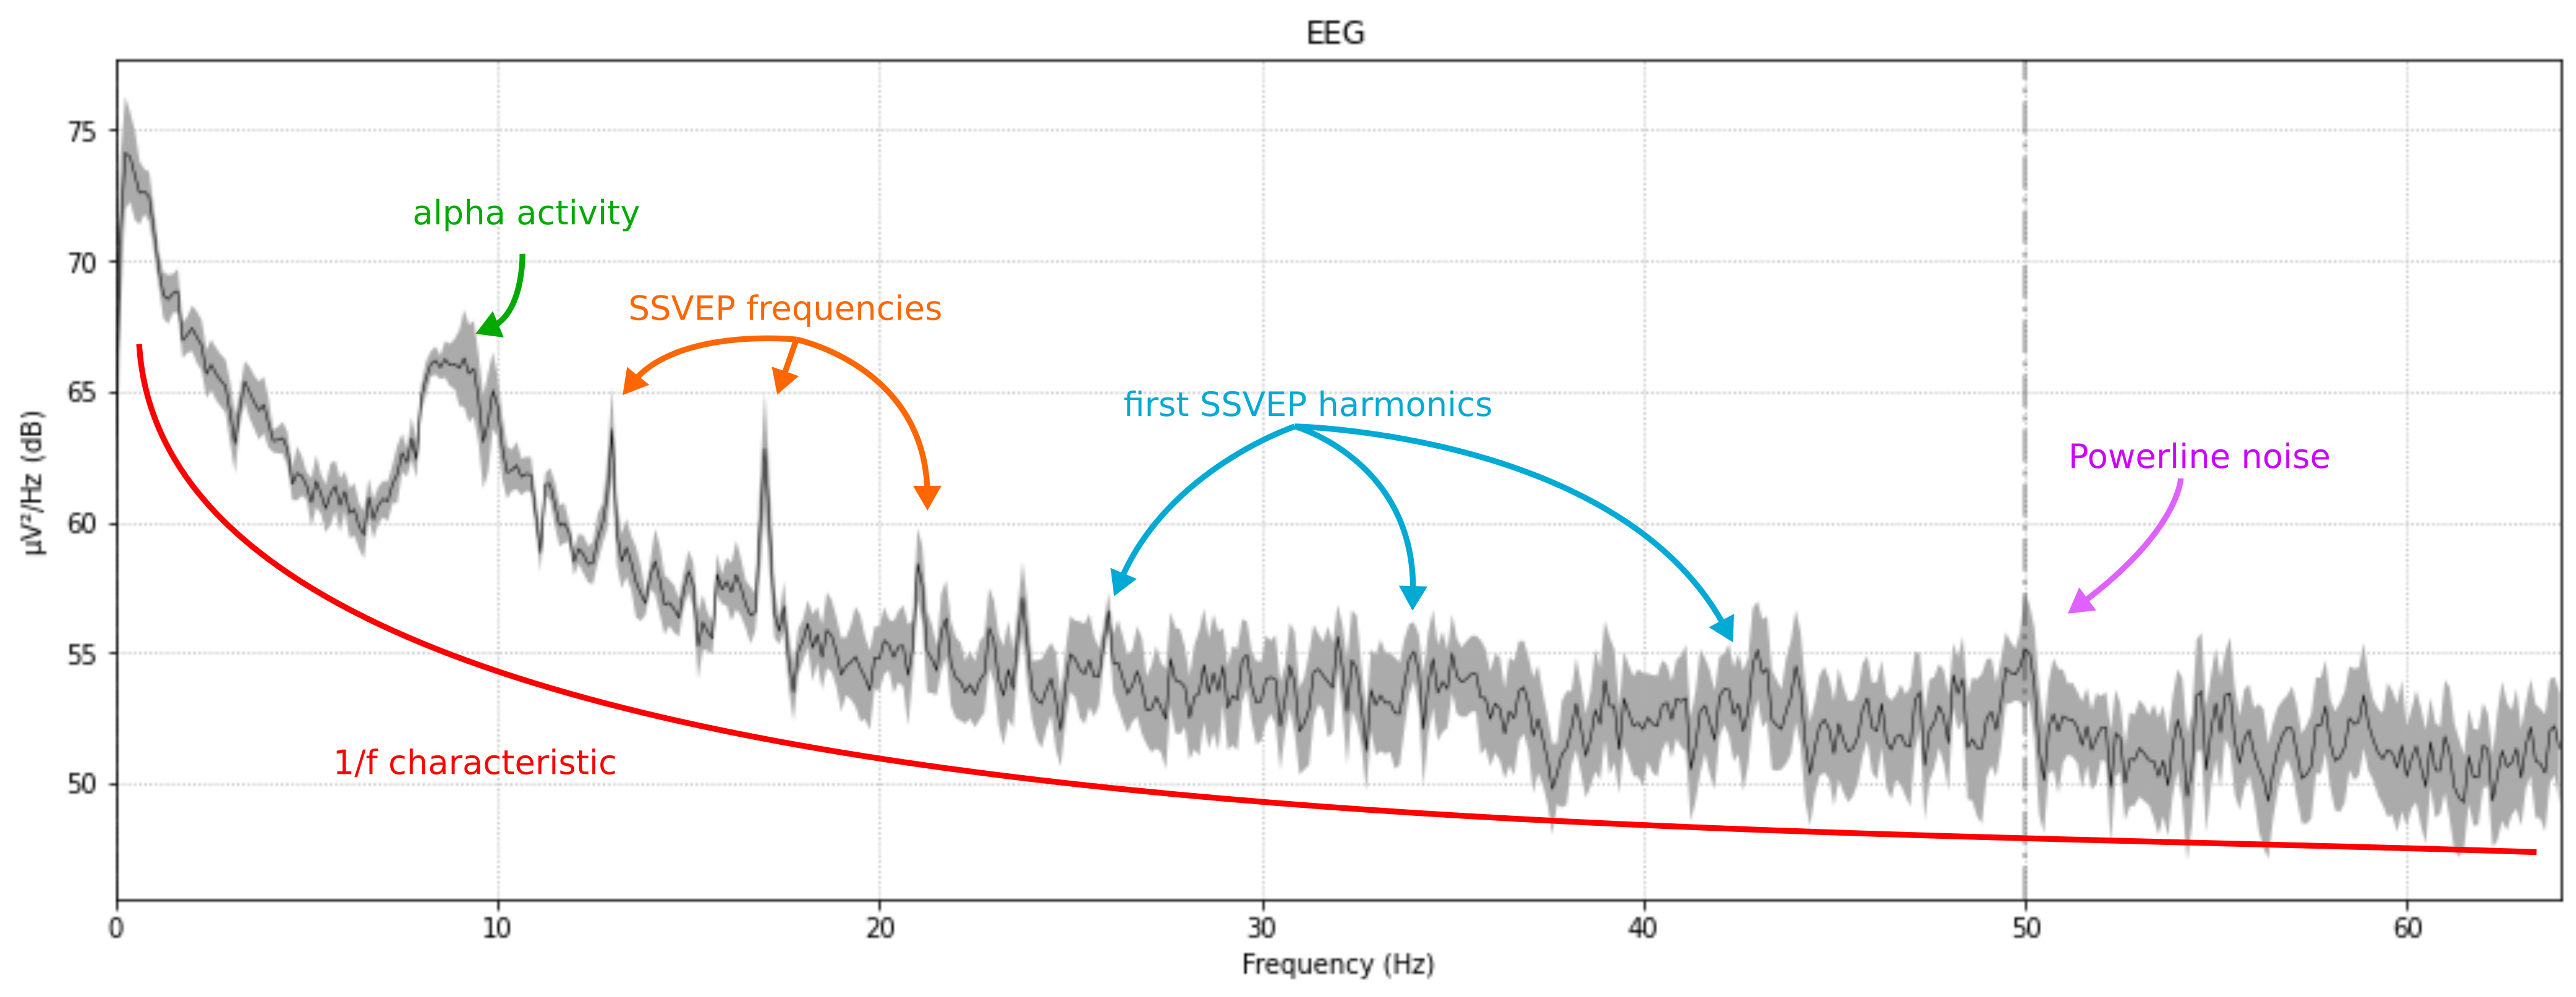
\includegraphics[width=\textwidth]{psd.png}
}

\frame{
	\frametitle{Choosing stimulation frequencies}
	\begin{changemargin}
		Consider
		\begin{itemize}
			\item SSVEP range (3.5-75Hz)
			\item Alpha activity (8-12Hz)
			\item Powerline frequency (EU: 50Hz, USA: 60Hz)
			\item Monitor refresh rate (60Hz, 144Hz, 240Hz, ...)
			\item Frequency spacing
			\item Comfort
		\end{itemize}

		\bigskip

		\textbf{Mind the harmonics!}
	\end{changemargin}
}


\end{document}
